\documentclass[12pt,a4paper,fleqn]{article}
\title{Progress Report}
\author{Syed Ahmad Raza}
\date{2017.11.01}
\usepackage{mathtools}
\usepackage{graphicx}
\usepackage{color}          % for color eps output
% \usepackage{afterpage}
\usepackage{float}          % to force a figure placement with [H] command
\usepackage{enumitem}
\usepackage{newtxtext}
\usepackage{newtxmath}
%\usepackage{layouts}       % for: \printinunitsof{in}\prntlen{\textwidth}

\begin{document}
\maketitle
\tableofcontents
\pagebreak

\section{Analytical solution of plane Poiseuille flow and 3D discretization of Navier-Stokes equation}

Ignoring the body force $\mathbf{f}$, the Navier-Stokes equation is represented by
\begin{equation}\label{eq:navier-stokes-no-f}
\frac {\partial \mathbf{u}}{\partial t} = -\frac{1}{\rho}\nabla p -\nabla \cdot (\mathbf{uu}) + \nu \nabla^2 \mathbf{u} \quad.
\end{equation}

\subsection{Analytical solution for 2D duct flow}
\begin{equation}\label{eq:analytical01}
\frac{U}{U_{\text{avg}}} = \frac{3}{2}\left[1-\left(\frac{y}{\tfrac{D}{2}}\right)^2\right] \quad,
\end{equation}
where
\begin{equation}\label{eq:analytical02}
U_{\text{avg}} = \frac{D^2}{12\mu}\left(-\frac{dP}{dx}\right) \quad,
\end{equation}
where the fraction \(\tfrac{dP}{dx}\approx\tfrac{\Delta P}{\Delta x}\) across the whole domain. Values of pressure are constant on the right edge of the domain where a Dirichlet pressure boundary condition has been selected. But on the left edge of the domain, where a Neumann boundary condition exists, the values vary from top to bottom and they have been averaged.

\begin{figure}[H]
	\centering
	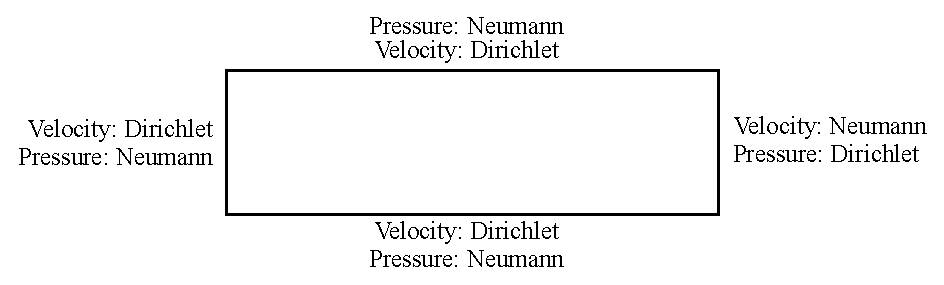
\includegraphics[width=0.95\textwidth]{boundary_conditions.eps}
	\caption{Velocity and pressure boundary conditions at each boundary of the domain are labeled.}
	\label{fig:boundary-conditions}
\end{figure}

\subsection{Calculation of \(L_2\) norm}
\begin{equation}\label{eq:l2norm}
L_2 \text{ norm} = \sqrt{\frac{\sum\limits_{i=1}^{n_y/2}\left(U_a - U_n\right)^2}{n_y/2}} \quad,
\end{equation}
where \(U_a\) is the value \(u\)-velocity value at the node from the analytical solution, whereas \(U_n\) is the velocity at the same node determined from the numerical solution, and \(n_y\) is the number of grid points on the \(y\)-axis.

\subsection{Discretization of the convective and diffusive terms for 3D domain}
The convective and diffusive terms can be discretized using the individual components. To apply the projection method, the equation \eqref{eq:navier-stokes-no-f} for the $u$-component can be written as
\begin{equation} \label{eq:3D-convective-diffusive-u}
\frac{\partial u}{\partial t} = -\frac{\partial uu}{\partial x} -\frac{\partial uv}{\partial y} -\frac{\partial uw}{\partial z} + \nu\left[\frac{\partial^2u}{\partial x^2} + \frac{\partial^2u}{\partial y^2} + \frac{\partial^2u}{\partial z^2}\right] \quad,
\end{equation}
which can be discretized as
\begin{align}\label{eq:3D-discretized_convective-diffusive-u}
\frac{\partial u}{\partial t} =
{}& - \frac{u_e^2 - u_w^2}{\Delta x} - \frac{u_n v_n - u_s v_s}{\Delta y} - \frac{u_o w_o - u_i w_i}{\Delta z}\\
& + \nu\left[
\left\{
\frac{u_{i+1,j,k} - u_{i,j,k}}{x_{i+2}-x_{i+1}}
- \frac{u_{i,j,k} - u_{i-1,j,k}}{x_{i+1}-x_i}
\right\}
\frac{1}{\Delta x}
\right.\nonumber\\
& + \left\{
\frac{u_{i,j+1,k} - u_{i,j,k}}{(y_{j+2}-y_j)/2}
- \frac{u_{i,j,k} - u_{i,j-1,k}}{(y_{j+1}-y_{j-1})/2}
\right\}
\frac{1}{\Delta y}
\nonumber\\
& \left. + \left\{
\frac{u_{i,j,k+1} - u_{i,j,k}}{(z_{k+2}-z_k)/2}
- \frac{u_{i,j,k} - u_{i,j,k-1}}{(z_{k+1}-z_{k-1})/2}
\right\}
\frac{1}{\Delta z}
\right] \quad ,
\end{align}
where, for the \emph{diffusion terms}, second-order central scheme has been used. Similarly for the \(v\)- and \(w\)-components, equation \eqref{eq:navier-stokes-no-f} will be
\begin{equation} \label{eq:3D-convective-diffusive-v}
\frac{\partial v}{\partial t} = -\frac{\partial vu}{\partial x} -\frac{\partial vv}{\partial y} -\frac{\partial vw}{\partial z} + \nu\left[\frac{\partial^2v}{\partial x^2} + \frac{\partial^2v}{\partial y^2} + \frac{\partial^2v}{\partial z^2}\right]
\end{equation}
and 
\begin{equation} \label{eq:3D-convective-diffusive-w}
\frac{\partial w}{\partial t} = -\frac{\partial wu}{\partial x} -\frac{\partial wv}{\partial y} -\frac{\partial ww}{\partial z} + \nu\left[\frac{\partial^2w}{\partial x^2} + \frac{\partial^2w}{\partial y^2} + \frac{\partial^2w}{\partial z^2}\right] \quad,
\end{equation}
which can be and discretized as
\begin{align}\label{eq:3D-discretized_convective-diffusive-v}
\frac{\partial v}{\partial t} =
{}& - \frac{v_e u_e - v_w u_w}{\Delta x} - \frac{v_n^2 - v_s^2}{\Delta y} - \frac{v_o w_o - v_i w_i}{\Delta z}\\
& + \nu\left[
\left\{
\frac{v_{i+1,j,k} - v_{i,j,k}}{(x_{i+2}-x_{i})/2}
- \frac{v_{i,j,k} - v_{i-1,j,k}}{(x_{i+1}-x_{i-1})/2}
\right\}
\frac{1}{\Delta x}
\right.\nonumber\\
& + \left\{
\frac{v_{i,j+1,k} - v_{i,j,k}}{y_{j+2}-y_{j+1}}
- \frac{v_{i,j,k} - v_{i,j-1,k}}{y_{j+1}-y_j}
\right\}
\frac{1}{\Delta y}
\nonumber\\
& \left. + \left\{
\frac{v_{i,j,k+1} - v_{i,j,k}}{(z_{k+2}-z_k)/2}
- \frac{v_{i,j,k} - v_{i,j,k-1}}{(z_{k+1}-z_{k-1})/2}
\right\}
\frac{1}{\Delta z}
\right] \quad
\end{align}
and
\begin{align}\label{eq:3D-discretized_convective-diffusive-w}
\frac{\partial w}{\partial t} =
{}& - \frac{w_e u_e - w_w u_w}{\Delta x} - \frac{w_n v_n - w_s v_s}{\Delta y} - \frac{w_o^2 - w_i^2}{\Delta z}\\
& + \nu\left[
\left\{
\frac{w_{i+1,j,k} - w_{i,j,k}}{(x_{i+2}-x_{i})/2}
- \frac{w_{i,j,k} - w_{i-1,j,k}}{(x_{i+1}-x_{i-1})/2}
\right\}
\frac{1}{\Delta x}
\right.\nonumber\\
& + \left\{
\frac{w_{i,j+1,k} - w_{i,j,k}}{(y_{j+2}-y_j)/2}
- \frac{w_{i,j,k} - w_{i,j-1,k}}{(y_{j+1}-y_{j-1})/2}
\right\}
\frac{1}{\Delta y}
\nonumber\\
& \left. + \left\{
\frac{w_{i,j,k+1} - w_{i,j,k}}{z_{k+2}-z_{k+1}}
- \frac{w_{i,j,k} - w_{i,j,k-1}}{z_{k+1}-z_k}
\right\}
\frac{1}{\Delta z}
\right] \quad.
\end{align}

\subsection{Poisson equation of pressure}
The Poisson equation of pressure in 3D may be written as
\begin{equation} \label{eq:3D-poisson-components}
\frac{\partial^2 p}{\partial x^2} + \frac{\partial^2 p}{\partial y^2} + \frac{\partial^2 p}{\partial z^2}
= \frac{1}{\Delta t} \left(\frac{\partial u^*}{\partial x} + \frac{\partial v^*}{\partial y} + \frac{\partial w^*}{\partial z}\right) \quad.
\end{equation}
Pressure may be found from the following discretized equation,
\begin{align}
p_{i,j,k}^{n+1} =
&\frac{1}{\left[ - \frac{Dy}{Dx1} - \frac{Dy}{Dx2} - \frac{Dy}{Dz1}- \frac{Dy}{Dz2} - \frac{Dx}{Dy1} - \frac{Dx}{Dy2} - \frac{Dx}{Dz1} - \frac{Dx}{Dz2} - \frac{Dz}{Dx1} - \frac{Dz}{Dx2} - \frac{Dz}{Dy1} - \frac{Dz}{Dy2}\right]}
\nonumber \\
&\times
\left[
- \frac{Dz}{Dx1}p_{i+1,j,k} - \frac{Dz}{Dx2}p_{i-1,j,k} - \frac{Dz}{Dy1}p_{i,j+1,k} - \frac{Dz}{Dy2}p_{i,j-1,k} \right.
\nonumber \\
&- \frac{Dy}{Dx1}p_{i+1,j,k} - \frac{Dy}{Dx2}p_{i-1,j,k} - \frac{Dy}{Dz1}p_{i,j,k+1} - \frac{Dy}{Dz2}p_{i,j,k-1}
\nonumber \\
&- \frac{Dx}{Dy1}p_{i,j+1,k} - \frac{Dx}{Dy2}p_{i,j-1,k} - \frac{Dx}{Dz1}p_{i,j,k+1} - \frac{Dx}{Dz2}p_{i,j,k-1}
\nonumber \\
&\left.
+ \frac{1}{\Delta t}\left\{
\left(u^*_{i,j,k}-u^*_{i-1,j,k}\right) \Delta y \Delta z
+ \left(v^*_{i,j,k}-v^*_{i,j-1,k}\right) \Delta x \Delta z
+ \left(w^*_{i,j,k}-w^*_{i,j,k-1}\right) \Delta x \Delta y
\right\}
\right]
\quad .
\end{align}

\end{document}
